\chapter{Anforderungsanalyse}
\label{sec:requirements}
% Wie ist die Ausgangslage (in Bamberg)? Wie werden/wurden die Anforderungen aufgestellt, 
% wer sind die Stakeholder und warum? Dann Anforderungen definieren und priorisieren
Bevor mit der eigentlichen Implementierung begonnen werden kann, ist es notwendig, die Anforderungsanalyse durchzuführen, da die Implementierung auf dieser basieren soll. Der erste Schritt hierzu besteht daraus, die Ausgangslage in Bamberg zu untersuchen, um darauf aufbauend die Stakeholder zu identifizieren, da diese den Ursprung der Anforderungen darstellen. Nachdem das Aufstellen der Anforderungen erfolgreich gewesen ist, können diese priorisiert und auf ihre Validität und ihre Realisierbarkeit analysiert werden. Basierend auf den Anforderungen werden dann User Stories abgeleitet, die die Anforderungen in einer konkreten Situation aus Sicht der Nutzenden beschreiben. Im Anschluss werden Use Cases präsentiert, um die von außen sichtbare Interaktion mit dem System zu beschreiben.

\section{Ausgangslage in Bamberg}
\label{sec:ausgangslage}
Bamberg\sidenote{\url{https://www.stadt.bamberg.de/Unsere-Stadt/Stadtinfo/}} ist eine kreisfreie Stadt in Bayern im Regierungsbezirk Oberfranken mit einer Einwohnerzahl von knapp 80.000 Einwohnern (Stand: Dezember 2022). Und auch wenn es sich bei Bamberg um eine Mittelstadt\sidenote{Klassifikation einer Stadt mit mindestens 20.000 und maximal 100.000 Einwohnern} handelt, können die Auswirkungen des Klimawandels auch hier beobachtet werden: Die Stadt Bamberg gibt an\sidenote{Diese Angaben sind aus einem persönlichen E-Mail Verkehr mit dem Klima- und Umweltamt der Stadt Bamberg zur Verfügung gestellt. Die angegebenen Daten dürfen in Arbeiten und Analysen eingebunden und veröffentlicht werden, die Inhalte und beigefügte Dateien des E-Mail Verkehrs allerdings nicht.}, dass sich seit 1990 der Energieverbrauch und die dadurch resultierenden Emissionen von etwa 2.162 MWh und 925.490 Tonnen CO2eq\sidenote{Formelzeichen für das Treibhauspotenzial} bis 2020 um etwa 30\% auf 2.035 MWh und 618.860 Tonnen CO2eq verringert haben, trotz steigender Einwohnerzahl \cite{Wehner2016}. Zurückzuführen ist dieser Abwärtstrend auf den Umstieg von konventionellen Energieträgern wie Kohle auf erneuerbare Energieträger\sidenote{Solarthermie und Biomasse}. Die Bilanzierung nach Sektoren zeigt, dass der gewerbliche Sektor (Industrie, Gewerbe, Handel und Dienstleistungen) in Bamberg etwa 53\% des Energieverbrauches einnimmt, während der private Sektor (private Haushalte, kommunale Einrichtungen und Verkehr) etwa 47\% beträgt. Der Anteil des gewerblichen Sektors ist damit deutlich höher als der Bundesdurchschnitt mit 44\%. \\ Die Auswirkungen dieser Zahlen erstrecken sich dabei von einer erhöhten Anzahl an Blaualgen in Badeseen, einem sinkenden Grundwasserspiegel und vertrockneten Bäumen\sidenote{Laut Angaben der Stadt vertrocknen die Rotbuchen im Hain}, bis hin zur Ausbreitung heimischer, aber auch neuer gesundheitsgefährdender Pflanzen und Tiere\sidenote{z.B. Zecken, Asiatische Tigermücke, Eichenprozessionsspinner, Ambrosia}. 

Die Fläche der kartierten Biotope\sidenote{Hier werden Lebensräume in einem bestimmten Gebiet erfasst und hinsichtlich ihrer Bedeutung für den Naturhaushalt bewertet. Der Anteil repräsentiert dabei das Verhältnis des Biotops zu der gesamten Stadt. In dieser Arbeit wird das Biotop \enquote{Flora} betrachtet, welches die Grünflächen in Bamberg darstellt.} in Bamberg hat 2019 etwa 13,3\% betragen, während dieser Wert 1998 noch bei 10,2\% lag. Diese Biotope sind gesetzlich geschützt, weswegen (erhebliche) Eingriffe in diese genehmigungspflichtig sind. Da für den Schutz verschiedene Zuständigkeiten\sidenote{Europäische Schutzgebiete unter der \ac{FFH-Richtlinie}, 
Naturschutzgebiete, Landschaftsschutzgebiete, Geschützte Landschaftsbestandteile, gesetzlich geschützte Biotope} existieren, kann eine rechtlich abgesicherte Gesamtnaturschutzfläche von insgesamt 32,5\% für das Stadtgebiet Bambergs angegeben werden. Durch politische Schlüsse und vorliegende Anträge ist geplant, die Schutzgebietsflächen in der gesamten Stadt zu vergrößern. 

Aufgrund dessen hat sich die Stadt Bamberg als Klimaziel gesetzt, bis 2035 zu 100\% auf erneuerbare Energieträger zu setzen und das Voranschreiten des Klimawandels zu verlangsamen.

Die Stadt selbst kann dabei in sogenannte \ac{LCZ}, also Klassifikationen, welche sich durch die logische Aufteilung einer Landschaft ergeben \cite{stewart2011local}, unterteilt werden. Zusammen mit dem Domänenwissen des Meteorologen Prof.\ Dr.\ Thomas Foken (vgl. Kapitel \ref{sec:stakeholder}) hat eine rudimentäre Unterteilung in sechs \ac{LCZ} stattgefunden: Die Innenstadt, die ERBA, Gartenstadt, Bamberg-Ost, der Hain, am Laubanger und das Berggebiet (siehe Abbildung \ref{fig:lcz}). Die Entscheidung über die Grenzen und der Gebiete erfolgt dabei durch die in der Literatur gegebenen Charakteristika, welche zum Definieren von \ac{LCZ} notwendig sind \cite{oke2004initial, stewart2012local}:

\keyword{Innenstadt (2)} -- Die Innenstadt kann als \enquote{Compact midrise} klassifiziert werden. Charakteristisch für diese \ac{LCZ} ist der dichte Mix aus mittelhohen Gebäuden, das Vorhandensein von wenigen bis keinen Bäumen und hauptsächlich asphaltierten Landflächen. Überwiegend lassen sich Stein, Ziegel, Kacheln und Beton als Baumaterialien vorfinden.

\keyword{ERBA (6)} -- Die ERBA kann als \enquote{Open low-rise} klassifiziert werden. In einem solchen befinden sich in der Regel flache Gebäude, die in einer offeneren Struktur angeordnet sind. Die Landflächen sind asphaltiert, weisen aber auch Grünflächen in Form von kleinen Pflanzen oder verstreuten Bäumen auf. Die Baumaterialien sind ähnlich wie in der Innenstadt, jedoch kann man an der ERBA häufig Holz als Baumaterial vorfinden.

\keyword{Gartenstadt (6B)} -- Die Gartenstadt ist wie die ERBA ein \enquote{Open low-rise}. Allerdings kann hier der Zusatz \textit{\enquote{B}} als \enquote{Land cover type}\sidenote{Nach \cite{stewart2012local}: Klassifikationen zu saisonalen Eigenschaften, wie z.B. schneebedeckter Boden, trockener/feuchter Boden etc.} zur Klassifikation hinzugefügt werden, welche nach \cite{stewart2012local} bedeutet, dass die Landschaft rege mit immergrünen Bäumen bestückt ist. Die Landflächen weisen zu einem Großteil Grünflächen mit kleinen Pflanzen auf. Diese Arten von \ac{LCZ} werden in der Regel für Wälder oder Stadtparks verwendet.

\keyword{Bamberg-Ost (3)} -- Der Osten Bambergs wird als \enquote{Compact low-rise} klassifiziert. Dieser weist die identischen Charakteristika wie die Bamberger Innenstadt auf, mit dem einzigen Unterschied, dass es sich bei den Gebäuden um niedrige Gebäude handelt.

\keyword{Hain (5)} -- Der Hain befindet sich in der Klasse des \enquote{Open midrise}. Dieser weist die identischen Charakteristika wie die ERBA auf, mit dem einzigen Unterschied, dass es sich bei den Gebäuden um mittelhohe Gebäude handelt und statt Holz überwiegend Beton und Stahl als Baumaterialien eingesetzt werden.

\keyword{Laubanger (8)} -- Der Laubanger wird in Bamberg als \enquote{Large low-rise} eingestuft. In dieser Klasse lassen sich in der Regel große, aber flache Gebäude in einer offeneren Struktur vorfinden. Bäume oder Grünflächen sind meistens nicht bis kaum vorhanden, da die Straßen und Wege überwiegend asphaltiert sind. Als Baumaterialien kommen häufig Stahl, Beton und Stein zum Einsatz.

\keyword{Berggebiet (6A)} -- Das Bamberger Berggebiet ähnlich wie die Gartenstadt und ERBA als \enquote{Open low-rise} eingestuft und weist die identischen Charakteristika auf. Der Zusatz \textit{\enquote{A}} besagt hierbei, dass eine große bzw. dichte Menge an Bäumen in der Landschaft vorzufinden ist, was in der Regel auch für Wälder oder Stadtparks zutrifft.

\begin{figure}[t] % [t]: place at top of page (recommended)
    \centering
    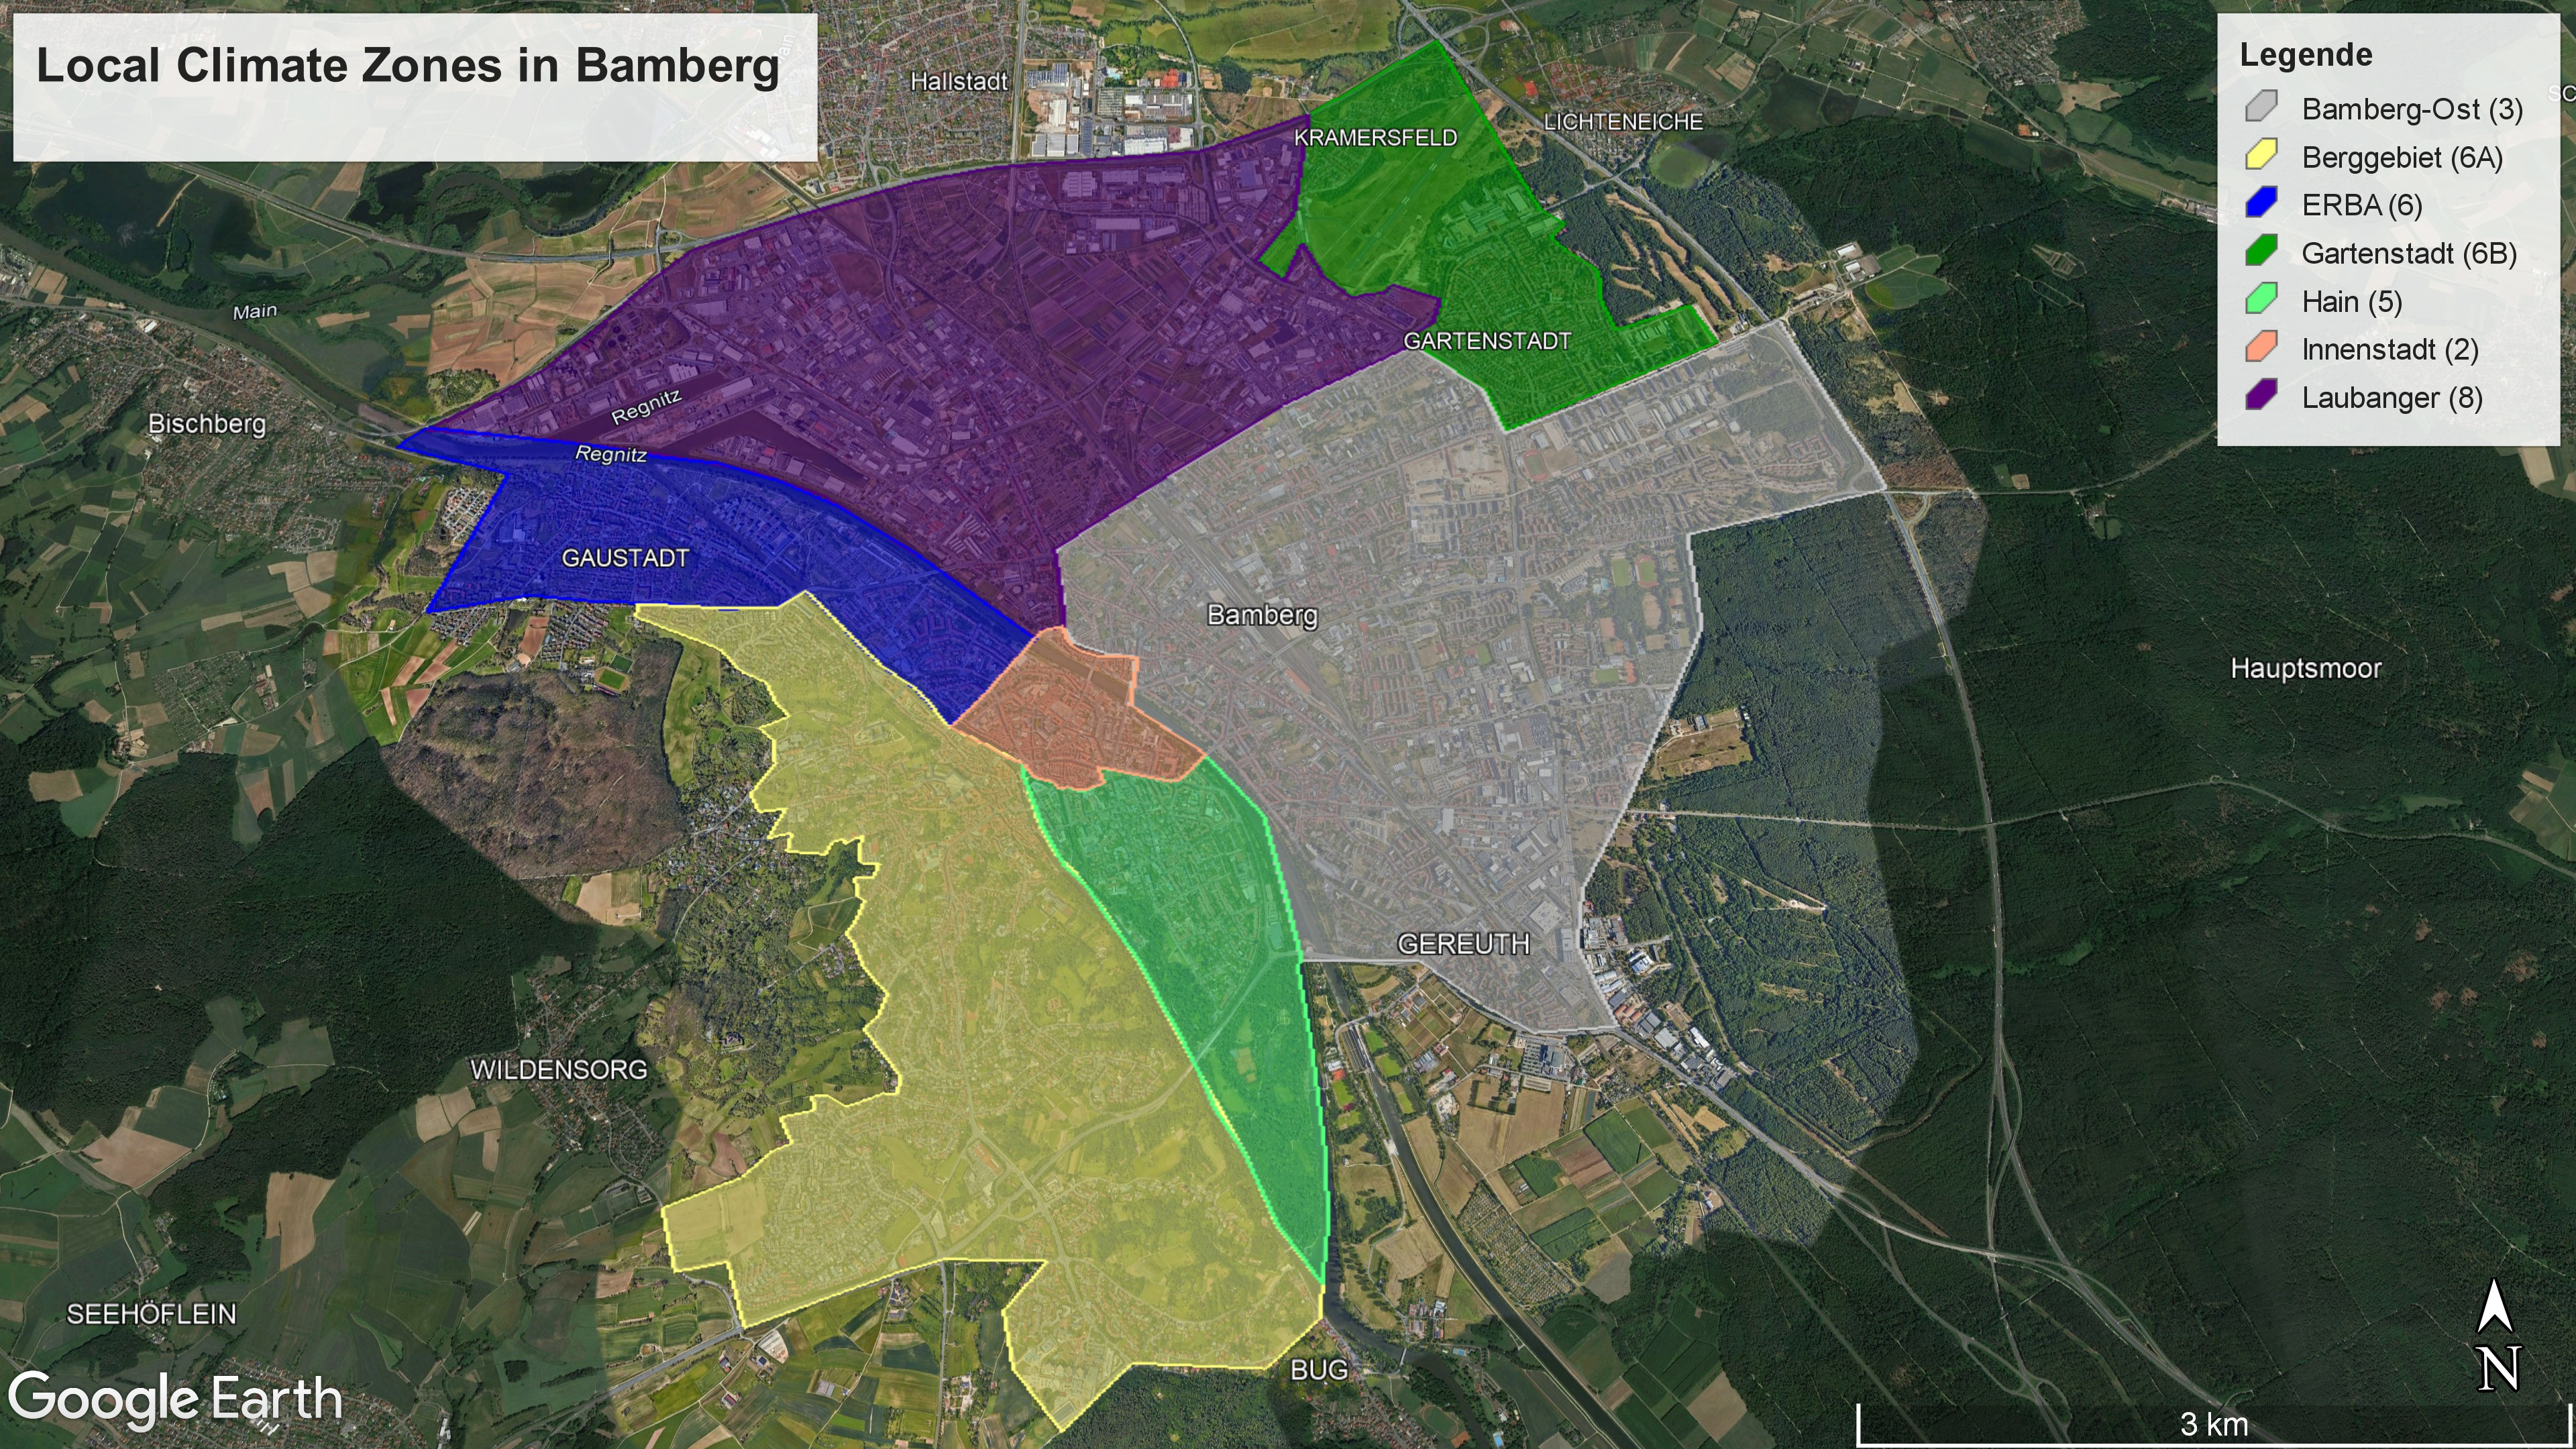
\includegraphics[width=1\textwidth]{figures/lcz.jpg}
    \decoRule
    \caption[LCZ in Bamberg]{Die sechs \ac{LCZ} in Bamberg (eigene Darstellung, basierend auf \cite{stewart2012local,oke2004initial})}
    \label{fig:lcz}
\end{figure}

Durch die Unterteilung der Stadt Bamberg in \ac{LCZ} ist es möglich, die Auslesungen der Wetterstationen und die Unterschiede der Messwerte in den einzelnen Gebieten nachvollziehen und damit besser analysieren zu können. \\ In der Stadt selbst sind Wetterstationen\sidenote{Die genaue Anzahl der Sensoren ist unbekannt, da nicht alle öffentlich einsehbar sind (Stand Oktober 2023: 42 Wetterstationen einsehbar} verteilt, die jeweils die Temperatur und Luftfeuchtigkeit am entsprechenden Standort messen. Auf der Wetterkarte von Netatmo\sidenote{\url{https://weathermap.netatmo.com/}} sind diese Auslesungen von öffentlichen Netatmo-Wetterstationen einsehbar.

\subsection{Identifikation der Stakeholder}
\label{sec:stakeholder}
In diesem Abschnitt der Arbeit werden die Stakeholder identifiziert, dessen Bedürfnisse und Ansprüche durch die Entwicklung des interaktiven Werkzeuges befriedigt werden sollen. Diese werden im Folgenden vorgestellt:

\paragraph{Der Bürgerverein Bamberg Mitte e.V.}
Bei dem \ac{BVM} handelt es sich um einen Bürgerverein in der Stadt Bamberg, welcher 1905 gegründet wurde und mit zahlreichen Projekten\sidenote{\url{https://bvm-bamberg.de/de/projektseiten/projekte-und-aktivitaeten/}} und durch das Praktizieren von Bürgerbeteiligung die Stadt Bamberg, vor allem in Hinblick auf die Stadtplanung und des Umwelt- und Denkmalschutzes, mitgestaltet\sidenote{\url{https://bvm-bamberg.de/de/buergerverein/unser-verein/}}.

Eines dieser Projekte ist das \enquote{Klimamessnetz auf der Bamberger Inselstadt}. Hier wird seit Anfang 2022 mithilfe von insgesamt neun smarten Netatmo-Wetterstationen\sidenote{\url{https://shop.netatmo.com/de-de/weather/smart-weather-station/weatherstation}} (Stand: 21. Oktober 2023) ein Klimamessnetz im Bamberger Zentrum zum Messen der Temperatur und Luftfeuchtigkeit an den entsprechenden Standorten\sidenote{Standorte der smarten Wetterstationen (\ac{LCZ}): Steinertstraße (Innenstadt), Lange Straße (Innenstadt), Am Weidenufer (ERBA), Holzmarkt (Innenstadt), Promenadestraße (Innenstadt), Wetzelstraße (ERBA), Fischerei (Innenstadt), Frauenstraße (Innenstadt) und Hainstraße (Hain)} aufgebaut. \\ Aus den Messungen der Wetterstationen ergibt sich, dass sich die Bamberger Innenstadt im Vergleich zu anderen \ac{LCZ} kaum abkühlt und die Temperaturen sich häufig von der offiziellen Station des \ac{DWD} unterscheiden (vgl. Webauftritt\sidenote{\url{https://bvm-bamberg.de/de/projektseiten/klima/}} des \ac{BVM}). Dies ist auch darauf zurückzuführen, dass das Fehlen von Bäumen und Grünflächen als Charakteristika eines \enquote{Compact mid-rise} ausschlaggebend für das Aufwärmen der Innenstadt ist: Ein Team von Geoökologen der Universität ETH Zürich hat in einer Studie gezeigt, dass Grünanlagen mit Bäumen in Städten zu einem Kühlungseffekt führen \cite{bastin2019global}. Dieser Effekt entsteht durch die Tatsache, dass Bäume durch ihre Wurzeln mehr Wasser aufnehmen können, welches im Umkehrschluss an trockenen und heißen Tagen verdunsten und so zu einer Abkühlung führen kann \cite{bastin2019global}. \\ Wie in Kapitel \ref{sec:methodologyrequirements} bereits erläutert, trifft sich der \ac{BVM} in regelmäßigen Abständen zum Analysieren der Auslesungen der Wetterstationen und Diskutieren von Maßnahmen, die zur Abkühlung der Innenstadt beitragen können. Durch die Teilnahme an diesen Treffen und die daraus resultierenden Gespräche mit den Mitgliedern des \ac{BVM} wurde in Erfahrung gebracht, dass das grundlegende Ziel des Vereins ist, Führungspersonen (z.B. in der Politik, Stadtplanung, Ämtern etc.) durch die Auslesungen der Wetterstationen zu sensibilisieren und damit zu einer Verbesserung der Lebensqualität durch das Erreichen des Kühlungseffektes in der Stadt Bamberg beizutragen. Dies soll ihrer Ansicht nach durch das Reduzieren von Parkplätzen (zum Minimieren von stehen gelassenen Autos) und Straßen für Autos erreicht werden, sodass für die neu geschaffenen Flächen Bäume und Grünflächen gepflanzt werden können.

\paragraph{Die Domänenexpert*innen}
Als Domänenexpert*innen werden in dieser Arbeit Personen definiert, die durch ihre Expertise und Erfahrung in einer Domäne wichtige Einblicke und Informationen, die über die Literatur hinausgehen, zu einem Projekt beitragen können. Sowohl für dieses Projekt, als auch für das Projekt des \ac{BVM} fungiert hier Prof.\ Dr.\ Thomas Foken\sidenote{\url{https://www.micrometeorology.de/}}, der durch seine Professur für Mikrometeorologie an der Universität Bayreuth langjährige Erfahrung in der (Mikro-)Meteorologie und der Klimaforschung besitzt. Durch die Teilnahme Prof.\ Dr.\ Fokens an den regelmäßigen Treffen mit dem \ac{BVM} ist es möglich gewesen, Erläuterungen und Definition der (Mikro-)Meteorologie zu erhalten, sodass erste Fokusse der Arbeit gesetzt werden konnten: \\ Einer dieser Punkte sind die sogenannten \enquote{Tropennächte}\sidenote{Nächte, in denen die minimale Temperatur zwischen 18 und 6 Uhr UTC mindestens 20°C betragen hat \cite{TropennachtDWD}} in Deutschland gewesen, die den Analysen des Professors nach eine deutliche Steigung in den letzten Jahren aufweisen. Dieser Aspekt ist insofern gefährlich für den Menschen, da der Körper des Menschen durch eine solche Hitzebelastung auf eine besondere Weise beansprucht wird und Probleme, die sich auf das Herz-Kreislaufsystem des Menschen auswirken, auftreten können \cite{Umweltbundesamt2023Hitze}. Tropennächte bieten sich insofern als guter Messwert an, da diese Kennzeichen für Hitzewellen in relativ kühleren Regionen der Welt (\textit{hier:} Deutschland) und für ihre eigentlich geringe Frequenz eine Ausnahmeerscheinung repräsentieren sollten, weswegen ein enger Zusammenhang zwischen Tropennächten und einer erhöhten Mortalität nachzuweisen ist \cite{fenner2015innerstadtische}.

\paragraph{Der \ac{MOBI}-Lehrstuhl}
Der \ac{MOBI}-Lehrstuhl\sidenote{\url{https://www.uni-bamberg.de/mobi/}} ist ein Lehrstuhl, welcher 2014 in der Fakultät Wirtschaftsinformatik und Angewandte Informatik an der Otto-Friedrich-Universität Bamberg angelegt wurde. Die Leitung übernimmt Prof.\ Dr.\ Daniela Nicklas, welche gleichzeitig die Betreuerin dieser Arbeit darstellt. Der Lehrstuhl beschäftigt sich insbesondere mit den \enquote{Fragen des Datenmanagements für mobile Systeme, Datenstrommanagement/komplexe Ereignisverarbeitung und der Unterstützung sensorbasierter Anwendungen, unter anderem im Bereich Smart Cities}. Die Hauptansprechpartner*innen im Rahmen dieser Arbeit sind Prof.\ Dr.\ Daniela Nicklas, Leonie Ackermann und Aboubakr El Hacen Benabbas gewesen. \\ Der MOBI hat ebenfalls an den regelmäßigen Treffen des \ac{BVM} zusammen mit Prof.\ Dr.\ Thomas Foken teilgenommen, sodass hier zusätzlich die Möglichkeit bestanden hat, Erfahrungen und Wissen aus dem Bereich der Informatik, der Datenverarbeitung und notwendige Schritte zum Entwickeln eines interaktiven Werkzeuges zu erhalten. Im gemeinsamen Austausch wurden Anforderungen ausgearbeitet, die sowohl für das \ac{BVM} und die Domänenexpert*innen in Hinblick auf die Auslesungen der Wetterstationen und die damit verbundenen Analysen der Sensordaten, als auch für den \ac{MOBI}-Lehrstuhl in Hinblick auf die technische Umsetzung relevant, aber auch realistisch sind.

\paragraph{Weitere Stakeholder}
Da eine Stadt selbst nicht als Stakeholder identifiziert werden kann, weil eine solche keine eigene Entscheidungs- bzw. Handlungseinheit darstellt, sollte Bamberg selbst trotzdem in diesem Abschnitt erwähnt werden. Dies ist darauf zurückzuführen, dass im Idealfall die eingesetzte Software Regierungsbehörden, Verwaltungen oder ähnliche Organisationen der Stadt erreichen kann und im Idealfall die Auswirkungen dieser Sache Bürger*innen, Unternehmen oder andere Interessensgruppen innerhalb der Stadt betreffen. Allerdings hat zum Zeitpunkt der Anforderungsanalyse weder mit der Stadt Bamberg, noch mit den Bürger*innen ein Austausch stattgefunden, sodass diese als indirekter Stakeholder erwähnt, aber weiterführend in dieser Arbeit nicht betrachtet werden.

Die in diesem Kapitel erläuterten Stakeholder wurden zum Zeitpunkt der Anforderungsanalyse identifiziert. Eine Limitierung auf diese Stakeholder ist aber nicht gegeben, sodass im Laufe der Arbeit oder in der Zukunft weitere Stakeholder identifiziert und in die Anforderungsanalyse aufgenommen werden können.
% \subsection{Das Bamberger Klimamessnetz als Grundlage der Sensordaten}

\section{Anforderungen}
In diesem Abschnitt der Arbeit werden die Anforderungen an das interaktive Werkzeug definiert. Diese werden in den folgenden Abschnitten erläutert und in einer Tabelle (vgl. \ref{sec:requirements_table}) zusammengefasst.

\subsection{Erfassung}
Die folgenden Anforderungen sind bei den Treffen mit den Stakeholdern erfasst worden. Eine Unterscheidung zwischen funktionalen\sidenote{Funktionale Anforderungen (FR) bestimmen spezifische Funktionen, Operationen oder Aufgaben, die eine Applikation (oder ihre Komponenten) ausführen muss, um die Bedürfnisse der Stakeholder zu erfüllen. Wenn das System die funktionalen Anforderungen nicht erfüllt, dann ist eine grundlegende Funktionalität des Systems nicht gegeben \cite{Puzhevich2021}} und nicht-funktionalen\sidenote{Nicht-funktionale Anforderungen (NFR) beschreiben Qualitätsmerkmale und Leistungsaspekte einer Applikation (oder ihrer Komponenten). Dabei handelt es sich nicht um spezifische Funktionen, sondern um die Art und Weise, wie diese Funktionen erbracht werden sollen \cite{Puzhevich2021}} Anforderungen wird hierbei getroffen, um diese besser zu strukturieren und priorisieren zu können. Eine Übersicht aller erfassten Anforderungen ist in der Tabelle \ref{sec:requirements_table} zu finden. Im weiteren Verlauf dieses Unterkapitels werden für eine citizen-science Anwendung typische\sidenote{Unterschieden wird dieser Aspekt dadurch, was eine typische Anwendung mit einem Crowdsensing-Ansatz von einer Anwendung ohne diesen unterscheidet (z.B. Login/Registrierung vs. Messen von Sensordaten in Echtzeit)} Anforderungen in der folgenden Form näher erläutert:

\textbf{Name der Anforderung (FR/NFR)}: Beschreibung und Begründung der Anforderung (\textit{Passform-Kriterium}; Priorität, wobei 1 die geringste und 5 die höchste Priorität darstellt)

\begin{enumerate}
    \item \textbf{Einsehen der Sensordaten in Echtzeit (FR)}: Die Nutzer*innen sollen die Möglichkeit haben, die Sensordaten in Echtzeit einsehen zu können. Dadurch soll es möglich sein, die Temperatur und Luftfeuchtigkeit an den entsprechenden Standorten zu betrachten und zu analysieren (\textit{Eine interaktive Karte mit den verschiedenen Stationen ist einsehbar und jede Station wird mit dem aktuellen Messwert der Temperatur und Luftfeuchtigkeit angezeigt}; 5)
    \item \textbf{Chatfunktionalität einer Station (NFR)}: Nach Wahl einer Station soll es möglich sein, eine Information an der gewählten Station zum gewählten Zeitpunkt zu hinterlassen. Der Grund dafür ist, dass Nutzende erkannte Anomalien eines ausgewählten Sensors erklären können (\textit{Textbox zur Eingabe des Chats erscheint nach Wahl einer Station und Zeitpunkt, Eingabe wird dauerhaft gespeichert}; 4)
    \item \textbf{Qualitätskontrolle der Sensordaten (NFR)}: Die Sensordaten sollen vor der Visualisierung mithilfe eines Algorithmus auf ihre Qualität überprüft und gefiltert werden. Dies soll durch das bestmögliche Entfernen von Ausreißern und das Ersetzen von fehlenden Werten erfolgen. Begründet ist dieser Aspekt dadurch, dass Fehler und Anomalien in den Sensordaten zu einer Verfälschung der Ergebnisse führen können (\textit{Qualitätskontrolle ist vor der Visualisierung der Sensordaten implementiert}; 4)
    \item \textbf{Speichern von Einstellungen (NFR)}: Die Einstellungen, die von den Nutzenden getätigt werden, sollen gespeichert werden, sodass diese beim nächsten Besuch der Anwendung wiederhergestellt werden können. Dadurch soll eine personalisierte Nutzung der Anwendung ermöglicht werden (\textit{Einstellungen werden in der Datenbank gespeichert und beim nächsten Besuch der Anwendung wiederhergestellt}; 4)
    \item \textbf{Vergleiche zwischen Stationen (NFR)}: Für Nutzende soll es möglich sein, mehrere Stationen auszuwählen und die Sensordaten der ausgewählten Stationen miteinander zu vergleichen, sodass Aussagen über das Klima, vor allem im Vergleich zwischen den \ac{LCZ}, getroffen werden können (\textit{Auswahl von mehreren Stationen ist zu gewünschten Zeitpunkten bzw. -fenstern ist möglich}; 4)
    \item \textbf{Heatmap (FR)}: Durch das Klicken eines Buttons soll es möglich sein, eine Heatmap der Temperatur und Luftfeuchtigkeit zu der eingeblendeten Karte der Stadt Bamberg zu aktivieren. Dadurch sollen Unterschiede zwischen den verschiedenen \ac{LCZ} sichtbar gemacht werden, um darauf basierend Rückschlüsse ziehen zu können (\textit{Heatmap wird durch Klicken eines Buttons aktiviert und die Temperatur und Luftfeuchtigkeit wird durch Farben dargestellt}; 3)
    \item \textbf{Einstellen des Zeitfensters für Stationen (NFR)}: Mithilfe verschiedener Auswahlmöglichkeiten soll die Anzeige der Auslesungen für die Stationen so manipuliert werden können, dass Auslesungen für unterschiedliche Zeiträume und -punkte angezeigt werden können. Dadurch sollen die Auslesungen im Verlauf der Zeit betrachtet werden können (\textit{Auswahlmöglichkeiten für die Anzeige der Auslesungen sind vorhanden, gewähltes Zeitfenster manipuliert entsprechend die Anzeige der Auslesungen}; 3)
    \item \textbf{Ein- und Ausblenden von Stationen (NFR)}: Es soll die Möglichkeit gegeben werden, einzelne (oder alle) Stationen ein- und auszublenden. Dadurch sollen nur für die Nutzenden relevante Stationen angezeigt werden, sodass eine Übersichtlichkeit auf der Karte ermöglicht wird (\textit{Ein- und Ausblenden von Stationen ist durch Button oder Klick auf entsprechende Stationen möglich}; 3)
    \item \textbf{Vordefinierte Standardsichten (NFR)}: Es sollen vordefinierte Standardsichten existieren, die Nutzende anklicken können, um entsprechende Ansichten auf der Karte zu erhalten. Dadurch können allgemein relevante Einstellungen, wie z.B. Sommertage, Tropennächte etc. schnell abgerufen werden (\textit{Vordefinierte Standardsichten sind vorhanden und können durch Klick auf entsprechende Buttons aktiviert werden}; 3)
    \item \textbf{Einsehen der eigenen Chats (NFR)}: Es soll die Möglichkeit geben, die eigenen Chats in denen die Nutzenden involviert sind, einzusehen. Dadurch soll eine Übersichtlichkeit über die eigenen Chats ermöglicht werden (\textit{Eigene Chats im Bereich \enquote{Mein Bereich} einsehbar}; 2)
    \item \textbf{Hinzufügen von Favoriten (NFR)}: Es soll die Möglichkeit geben, Stationen als Favoriten zu markieren, sodass diese in einem eigenen Bereich gespeichert werden können. Dadurch soll eine Übersichtlichkeit über die eigenen Favoriten ermöglicht werden (\textit{Favoriten können durch Klick auf entsprechende Stationen hinzugefügt werden und sind im Bereich \enquote{Mein Bereich} einsehbar}; 2)
    \item \textbf{Anzeigen von relevanten Landmarks auf der Karte (NFR)}: Es soll die Möglichkeit geben, (temperatur-)relevante Landmarks auf der Karte anzuzeigen. Diese sollen die ausgelesenen Sensordaten insofern unterstützen, sodass Zusammenhänge zwischen den Standorten der Stationen und den lokalen Gegebenheiten, wie z.B. Wasserbrunnen, Wälder etc. erschlossen werden können (\textit{(Temperatur-)relevante Landmarks sind auf der Karte dauerhaft einsehbar}; 2)
    \item \textbf{Einheitliche Datenverwaltung (NFR)}: Die Daten sollen in einer einheitlichen Datenbank verwaltet werden, da diese zum aktuellen Stand an unterschiedlichen Orten vorliegen und eine Übersicht erschweren (\textit{Daten liegen auf einer Datenbank vor und ein Zugriff auf diese ist möglich}; 1)
\end{enumerate}

Eine Limitierung der Anforderungen auf diese genannten ist nicht gegeben. Es ist möglich, dass im Laufe der Arbeit weitere Anforderungen hinzukommen oder bestehende Anforderungen angepasst werden.

\subsection{Priorisierung}
Die Priorisierung der Anforderungen erfolgt anhand der \textit{MoSCoW}-Methode\sidenote{MoSCoW ist ein Akronym für \textit{Must have, Should have, Could have, Won't have} und wird verwendet, um die Priorität von Anforderungen zu bestimmen \cite{clegg1994case}}. Eine Priorisierung erfolgt dabei durch die Abstimmung mit den Stakeholdern, wobei die Priorität anhand der folgenden Kriterien bestimmt wird:

\begin{itemize}
    \item \textbf{Must have (5)}: Anforderungen, die als \enquote{Must have} klassifiziert werden, sind essentiell für das Projekt und müssen umgesetzt werden, da diese für die Stakeholder von hoher Bedeutung sind.
    \item \textbf{Should have (4)}: Anforderungen, die als \enquote{Should have} klassifiziert werden, sind wichtig für das Projekt und sollten umgesetzt werden, da diese für die Stakeholder von hoher Bedeutung sind.
    \item \textbf{Could have (3-2)}: Anforderungen, die als \enquote{Could have} klassifiziert werden, sind wünschenswert für das Projekt und können umgesetzt werden, da diese für die Stakeholder von mittlerer Bedeutung sind.
    \item \textbf{Won't have (1)}: Anforderungen, die als \enquote{Won't have} klassifiziert werden, sind nicht relevant für das Projekt und werden nicht umgesetzt, da diese für die Stakeholder von geringer Bedeutung sind.
\end{itemize}

Unter den Kategorien \enquote{Must have} und \enquote{Should have} finden sich unter anderem auch Anforderungen, die für ein citizen-science Projekt essenziell sind, da dieser Aspekt den Fokus dieser Arbeit repräsentiert. Die Kategorien \enquote{Could have} und \enquote{Won't have} beinhalten Anforderungen, die bedeutend und wünschenswert für das Projekt sind, aber nicht zwingend umgesetzt werden müssen. 

\subsection{Analyse}
Aufgrund der Tatsache, dass unter den Stakeholdern auch Domänenexpert*innen, für sowohl die technische Umsetzung als auch für die Domäne der (Mikro-)Meteorologie lokalisiert werden können, befinden sich alle aufgestellten Anforderungen in einem realistischen Rahmen, wenn lediglich die allgemeine Realisierbarkeit betrachtet wird. Inwiefern die Anforderungen in der vorgegebenen Zeit umgesetzt werden können, wird bereits in Kapitel \ref{sec:umsetzung} erläutert. \\ Um den Crowdsensing-Ansatz dieser Arbeit zu erfüllen, und Rückschlüsse auf einen Mehrwert durch die Nutzung dieses Ansatzes zu ziehen, müssen entsprechende Anforderungen existieren und höher priorisiert sein. Dies wird erreicht durch die Anforderungen 

\begin{itemize}
    \item Chatfunktionalität einer Station
\end{itemize}

mit dessen Implementierung Nutzende aktiv Anomalien erkennen, markieren und im weiteren Verlauf eine Erklärung für den Ursprung dieser zu finden. Bevor es zu diesem Schritt kommen kann, muss die Umgebung für diesen Prozess gebaut werden. Dafür benötigt man die Anforderungen 

\begin{itemize}
    \item Einsehen der Sensordaten in Echtzeit
    \item Vergleiche zwischen Stationen
    \item Einstellen des Zeitfensters für Stationen
\end{itemize}

sodass eine Grundlage für das Verfassen einer Annotation gegeben ist. Um die Qualität der vorliegenden Daten und der Nutzenden-Erfahrung zu steigern, werden die Anforderungen 

\begin{itemize}
    \item Qualitätskontrolle der Sensordaten
    \item Speichern von Einstellungen
    \item Heatmap
    \item Ein- und Ausblenden von Stationen
    \item Vordefinierte Standardsichten
    \item Hinzufügen von Favoriten
    \item Anzeigen von relevanten Landmarks auf der Karte
    \item Einheitliche Datenverwaltung
\end{itemize}

aufgestellt. Aus dieser Aufzählung wird deutlich, dass das Ziel des Projektes, und damit des Crowdsensing-Ansatzes, klar durch das Vorhandensein einer Anforderung (Chatfunktionalität einer Station) definiert ist. Alle anderen aufgestellten Anforderungen stellen dabei nur Notwendigkeiten dar, dieses Ziel zu erreichen oder die Qualität des Endproduktes zu steigern. \\ Aufgrund dessen befinden sich die aufgestellten Anforderungen ebenfalls in einem validen Rahmen. Dies ist zusätzlich darauf zurückzuführen, dass das Projekt iterativen Prozessen unterliegt, sodass die Anforderungen nach jeder Iteration in Form der regelmäßigen Treffen mit den Stakeholdern angepasst werden können. Paradoxe, nicht-realisierbare oder den Rahmen sprengende Anforderungen werden mit den Stakeholdern evaluiert, sodass entsprechende Lösungen gebildet werden oder diese angepasst werden können, um Validität zu gewährleisten.

Inwieweit die Anforderungen dieses Projekts erfüllt sind, wird in Kapitel \ref{sec:requirements_evaluation} evaluiert. 

\section{User Stories}
Im folgenden werden User Stories beschrieben, um die Anforderungen an einem konkreten Beispiel zu repräsentieren. Die User Stories basieren dabei auf den Aussagen der Stakeholder aus den regelmäßigen Meetings, deren Bedürfnisse, Wünsche und Anregungen\sidenote{In Bezug auf das Klimamessnetz der Stadt Bamberg}, und sollen eine konkrete Vision für verschiedene Personen(-gruppen), welche durch die Entwicklung eines interaktiven Werkzeuges unterstützt wird, darstellen. Angelegt werden diese in der folgenden Form unter Verwendung der Vorlage von \cite{AmblerUserStory}:

\enquote{Als \textbf{<Rolle>} möchte ich \textbf{<Ziel/Wunsch>}, um \textbf{<Nutzen>}}

\begin{itemize}
    \item \textbf{Bürgerin der Stadt Bamberg}: Als Bürgerin der Stadt Bamberg möchte ich die Temperatur und Luftfeuchtigkeit an den verschiedenen Standorten in Echtzeit einsehen können, um die Auswirkungen des Klimawandels auf die Stadt Bamberg zu erkennen.
    \item \textbf{Mitglied des \ac{BVM}}: Als Mitglied des \ac{BVM} möchte ich die Temperatur und Luftfeuchtigkeit an den verschiedenen Standorten in der Innenstadt in Echtzeit einsehen und analysieren können, um die Auswirkungen der Bodenversiegelung\sidenote{Der Boden ist versiegelt, wenn dieser luft- und wasserdicht abgedeckt wird, z.B. durch Beton, Asphalt oder durch errichtere Gebäude \cite{UmweltbundesamtBodenversiegelung}} in der Bamberger Innenstadt zu erkennen.
    \item \textbf{Mitglied des \ac{ADFC} Bamberg}: Als Mitglied des \ac{ADFC} Bamberg möchte ich die Temperatur und Luftfeuchtigkeit an den verschiedenen Standorten in Bamberg untersuchen zu können, um die Auswirkungen des Autoverkehrs auf das Bamberger Klima zu erkennen.
    \item \textbf{Studierende der Informatik an der Universität Bamberg}: Als Studierender der Informatik an der Universität Bamberg möchte ich Werkzeuge für die Bamberger Bürger*innen schaffen, um das Bewusstsein für den Klimawandel zu stärken.
    \item \textbf{Lehrende der Informatik an der Universität Bamberg}: Als Lehrende der Informatik an der Universität Bamberg möchte ich Projekte unterstützen, die einen Mehrwert für die Bamberger Bürger*innen schaffen, um das Bewusstsein für den Klimawandel zu stärken.
    \item \textbf{Meteorologe in Bamberg} Als Meteorologe in Bamberg möchte ich die Stadt Bamberg über die Auswirkungen des Klimawandels informieren, um die Stadt Bamberg auf dem Weg zu einer klimafreundlicheren\sidenote{Mehr Grünflächen, erhöhte Anzahl von Bäumen und weniger versiegelte Böden} Stadt zu unterstützen.
\end{itemize}

\section{Use Cases}
Um auf eine simple Art und Weise aufzuzeigen, was die fertige Softwarelösung können muss, kann ein Use-Case-Diagramm (vgl. Abbildung \ref{fig:usecase_diagram}) eingesetzt werden. In diesem werden die Akteure (\textit{hier:} User und Administrator) und die entsprechenden Anwendungsfälle in Ellipsen dargestellt. Die Beziehungen der einzelnen Anwendungsfälle untereinander, aber auch mit den Akteuren wird durch gerichtete Graphen verdeutlicht. Das Rechteck repräsentiert das System und dessen Grenzen, in welchem sich die einzelnen Anwendungsfälle befinden. 

\begin{figure*}[t]
    \centering
    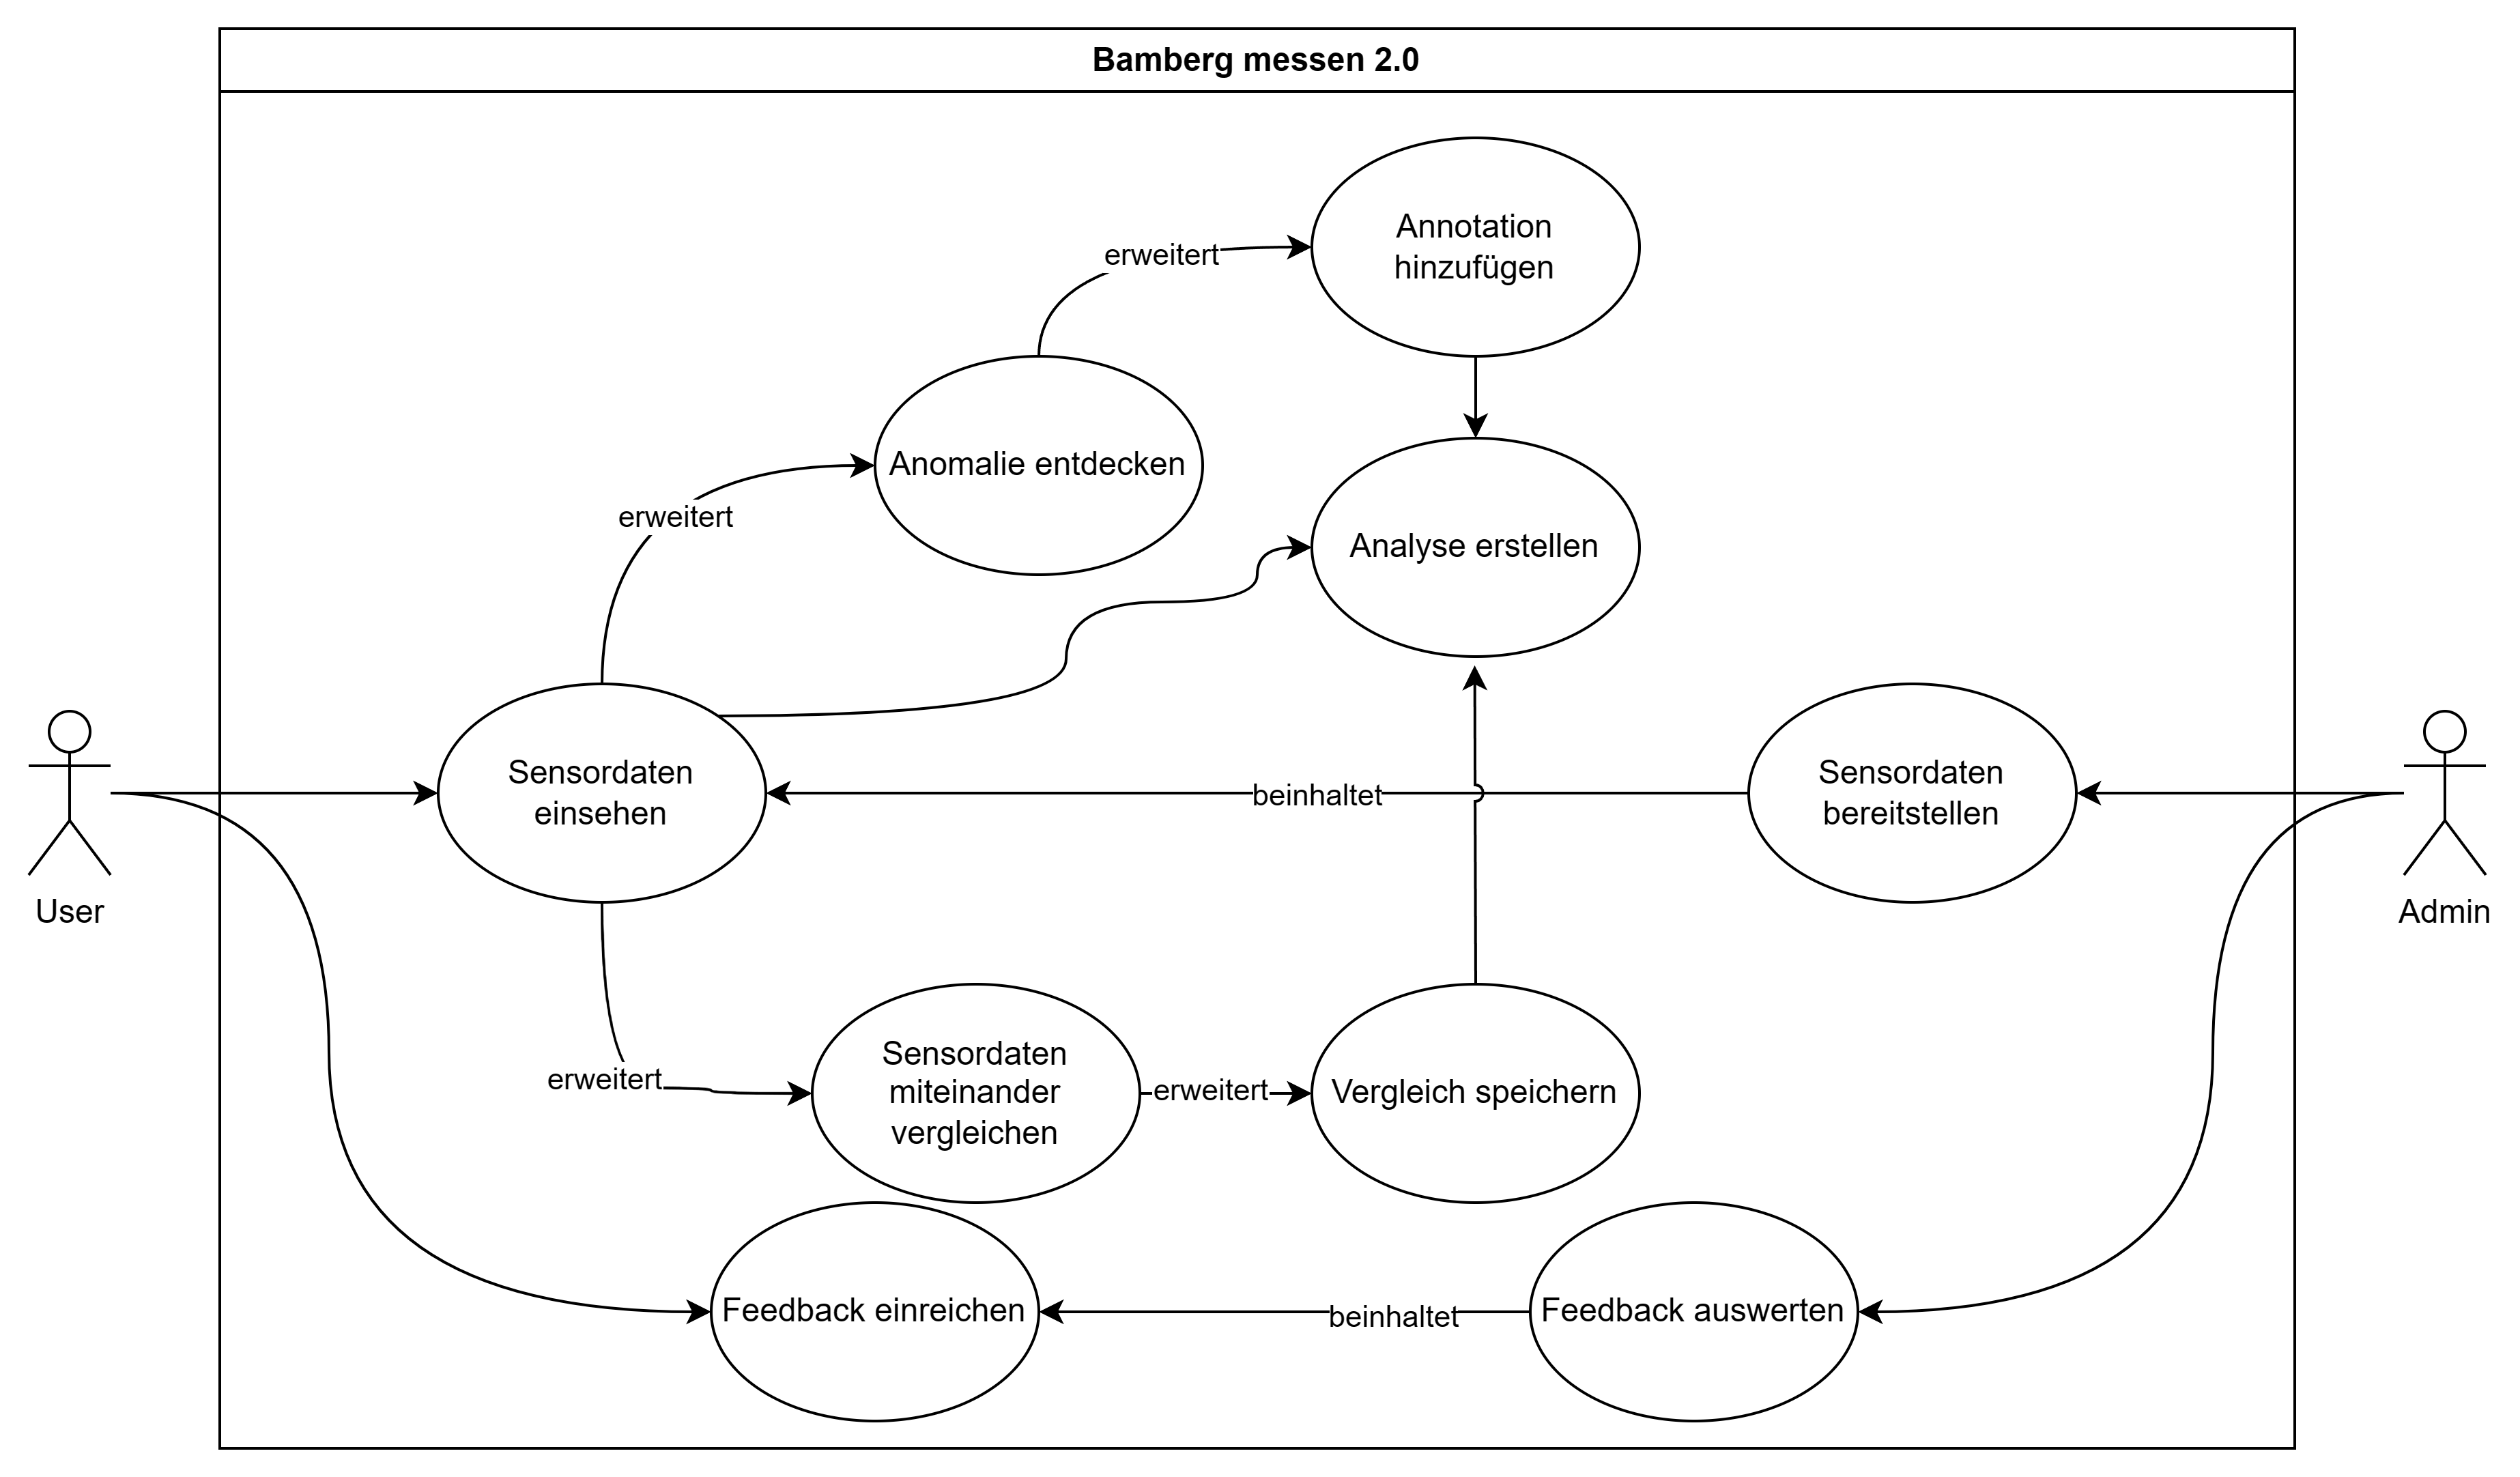
\includegraphics[width=1.5\textwidth]{figures/usecases.png}
    \decoRule
    \caption[Use-Case-Diagramm]{Use-Case-Diagramm}
    \label{fig:usecase_diagram}
\end{figure*}